La información de las organizaciones se considera un punto clave para la realización 
de muchos servicios de valor añadido tanto para la Administración Pública como 
para otras entidades. El conocimiento del estado financiero de una entidad, la actividad que ha desarrollado a 
través de proyectos, los productos y servicios ofertados, el listado de clientes y socios, etc., se considera una 
información de alto interés para la monitorización y la selección de posibles entidades 
para el establecimiento de relaciones de negocios. Desde el punto de vista interno de la propia organización, su estructura y 
personas implicadas en el desarrollo de la actividad de negocio así como la explotación del conocimiento organizacional 
son factores clave que determinan el camino a seguir por una entidad y su valor como tal. Como se ha señalado 
en la Sección~\ref{sect:orgs}, existen varios enfoques para la representación de la información de las organizaciones, 
en el caso objeto de estudio de este documento se centrará principalmente en los siguientes puntos: 1) información 
de contacto de la organización respecto a su localización y 2) persona de referencia para el establecimiento de 
relaciones. Este planteamiento es válido tanto para la representación de la información de los organismos que, cuentan con capacidad 
para la realización de contratos públicos, como para aquellos que deseen concursar a través de ofertas y cuya información 
debe perdurar a lo largo del tiempo hasta el fin del contrato. De acuerdo a la información disponible en las distintas 
fuentes de información de los anuncios de licitación las organizaciones o entidades modeladas cumplirán, al menos, con estos 
dos puntos clave que suponen un gran avance respecto a la información actual.

\subsection{Proceso de Producción de \linkeddata de Organizaciones}
Al igual que en el caso de las clasificaciones de productos y según la definición realizada 
de este proceso en la Sección~\ref{sect:produccion}, este proceso implica todas las tareas 
que se han de realizar para la transformación de un \dataset de entrada $\mathcal{G}$, mediante 
unas reglas de \textit{mapeo} $\mathcal{M}$, con el objetivo de conseguir un \dataset \gls{RDF} $\mathcal{D}$, de esta forma 
se define el método semántico de producción. 

\subsubsection{Tarea $t_1$-Análisis del \dataset a transformar}\label{t1-orgs}
Las organizaciones, tanto órganos contrantes como ofertantes, durante el proceso administrativo de 
contratación pública generan información y datos abarcando un amplio espectro, sin embargo para los fines 
de apertura y enlazado de datos mediante un modelo formal se considera 
suficiente la representación de la información de contacto de una entidad, 
incluyendo tanto a la persona física o jurídica de la misma con especial atención a su localización. La realidad 
es que la obtención de la información y datos pormenorizados de una organización se haya disponible públicamente, 
pero a través de fuentes información de difícil consulta que carecen de relevancia crítica para el estudio realizado en este trabajo, 
por ello se ha decidido realizar un primer acercamiento a la información empresarial focalizando el esfuerzo en la selección 
de un modelo formal que suministre el marco de trabajo adecuado para la representación de información 
de las organizaciones de una forma sencilla y operativa en el ámbito de la contratación pública 
electrónica. En este sentido, emergen tres entidades: organizaciones, personas y países, en las que 
hay que representar distintos datos, principalmente en las dos primeras información relativa a los datos de contacto y en la última 
la geolocalización. Una organización puede tener diferentes identificadores, asumiendo que cada uno de sus departamentos o 
subdivisiones y también las personas varían de acuerdo a la unidad mínima de organización seleccionada 
y en consecuencia su localización. La invariante que se produce reside en que para un proceso de contratación pública, la tupla 
una organización (entidad, departamento, división, etc.), una persona de contacto, un país y un propósito determinado es única.

En este sentido, surge la necesidad de especificar las organizaciones, personas, direcciones y países en un modelo formal. Para 
la utilización de un modelo formal, extensible que suministre el soporte necesario para el almacenamiento de la información y datos de las entidades con carácter 
multiling\"{u}e, se ha seleccionado la ontología ``\textit{Organizations}'' realizada por \textit{Dave Reynolds} (Epimorphics Ltd) ya que conjuga 
los esfuerzos de anteriores propuestas facilitando la representación de cualquier tipo de entidad desde un punto de vista 
estructural, información de contacto, actividad desarrollada, etc., convirtiéndose de esta manera en el marco de trabajo 
apropiado para el tratamiento de la información de licitantes y licitadores. La información sobre las personas se representa con la ontología 
FOAF, mientras que finalmente los países y su información, además de utilizar el \dataset de NUTS (regiones de Europa), reutilizan 
las definiciones realizadas en la DBPedia. 

La información que se tomará como paradigmática para este enfoque surge de las hojas de cálculo disponibles en el servidor 
\gls{FTP} de \gls{TED} en la Unión Europea, que consta de los siguientes campos: \textit{organisation official name, postal address (street), town, 
postalcode, countrycode, contact: attention, tel, fax, email, url, postal-code for the country (1 to 3 characters), contact point(s): telephone number, 
fax number, e-mail address, \gls{URL}}, un ejemplo completo se ha señalado en la Figura~\ref{fig:orgs-example-ted} extraído 
de la documentación oficial de TED. No obstante y de acuerdo a la ejecución del proyecto ``10ders Information Services'' se ha seleccionado 
el \dataset provisto por la empresa Gateway S.C.S., reseñado en la Figura~\ref{fig:orgs-example}, y consistente en $50,000$ entidades. La actualización 
de este \dataset es incremental a lo largo del tiempo y crece generando una gran masa de información de datos, con el objetivo de realizar la prueba 
de concepto de representación de la información empresarial, se ha decidido acotar a las necesidades del proyecto.

\begin{figure}[!htp]
\begin{lstlisting} 
<addr>
  <organisation>Westminster City Council</organisation>
  <address>City Hall, 64 Victoria Street</address>
  <contact>Westminster Accord</contact>
  <attention>Linda Pinder</attention>
  <countrycode>UK</countrycode>
  <town>London</town>
  <postalcode>SW1E 6QP</postalcode>
  <tel>020 7641 3173</tel>
  <email><txemail>lpinder@westminster.gov.uk</txemail></email>.
  <fax>020 7641 3017</fax>
</addr>
\end{lstlisting}
	\caption{Ejemplo de datos sobre una Organización en TED.}
	\label{fig:orgs-example-ted}
\end{figure}


\begin{figure}[!htp]
\begin{lstlisting} 
ID contrato, ISO code, campos internos de la BBDD, tipo de entidad, nombre entidad en cada idioma, dir. postal, campos de la dir. postal
...
000170-2011,da,false,7,5,1,ContractingAuthority,Europa-Parlamentet,,,"plateau de Kirchberg, 2929, Luxembourg",plateau de Kirchberg,2929,Luxembourg,,"",,,
000170-2011,lv,false,7,5,1,ContractingAuthority,Eiropas Parlaments,,,"plateau de Kirchberg, 2929, Luksemburga",plateau de Kirchberg,2929,Luksemburga,,"",,,
000170-2011,nl,false,7,5,1,ContractingAuthority,Europees Parlement,,,"plateau de Kirchberg, 2929, Luxemburg",plateau de Kirchberg,2929,Luxemburg,,"",,,
000170-2011,pl,false,7,5,1,ContractingAuthority,Parlament Europejski,,,"plateau de Kirchberg, 2929, Luksemburg",plateau de Kirchberg,2929,Luksemburg,,"",,,
000170-2011,pt,false,7,5,1,ContractingAuthority,Parlamento Europeu,,,"plateau de Kirchberg, 2929, Luxemburgo",plateau de Kirchberg,2929,Luxemburgo,,"",,,
000170-2011,es,false,7,5,1,ContractingAuthority,Parlamento Europeo,,,"plateau de Kirchberg, 2929, Luxemburgo",plateau de Kirchberg,2929,Luxemburgo,,"",,,
...
\end{lstlisting}
	\caption{Ejemplo de datos sobre Organizaciones.}
	\label{fig:orgs-example}
\end{figure}


\subsubsection{Tarea $t_2$-Limpieza de datos}
La oportunidad de reutilizar la información y datos suministrados por una empresa experta en el dominio de la 
contratación pública y con la capacidad para filtrar aquella información y datos relevantes resulta de gran 
valor para la ejecución de la transformación de estos datos. Es por ello que partiendo de este \dataset 
original, esta tarea ya ha sido realizada y los datos a transformar se encuentran en condiciones óptimas 
de calidad, tanto en contenido como en formato (\gls{CSV}).

\subsubsection{Tarea $t_3$-Selección de Vocabularios}
Los vocabularios seleccionados para modelar la información de las organizaciones teniendo en cuenta el análisis 
realizado en la tarea $t_1$ y la metodología seguida en los anteriores apartados se presentan en la Tabla~\ref{table:orgs-select-vocabs}. 
En general, se trata de vocabularios que atienden a los siguientes criterios:

\begin{enumerate}
 \item Formalización de una estructura taxonómica, como RDFS, \gls{SKOS} u \gls{OWL}.
 \item Realización de \textit{mapeos} entre conceptos, como SKOS y OWL.
 \item Representación de tipos de datos, como \gls{XML Schema}.
 \item Gestión de información multiling\"{u}e, como SKOS-XL y RDFS.
 \item Representación de información de negocio (entidades y personas), como ``\textit{Organizations Ontology}'', ``\gls{FOAF}'' y ``\textit{DBPedia Ontology}''.
 \item Adición de metadatos y provenance, como \textit{Dublin Core Terms}, \gls{voID} y \textit{Provenance Ontology}.
 \item Representación de información de contacto como vCard en RDF.
\end{enumerate}


\begin{longtable}[c]{|l|p{4cm}|p{4cm}|p{4cm}|} 
\hline
\textbf{Prefijo} &  \textbf{Vocabulario} &  \textbf{Fuente} & \textbf{Uso} \\\hline
\endhead
 dbpedia & \url{http://dbpedia.org/ontology/}&  Comunidad \linkeddata. & Reutilización de definiciones. \\ \hline 
 dc & \url{http://purl.org/dc/elements/1.1/}&  \textit{Dublin Core Metadata Initiative} & Creación de metadatos para los documentos. \\ \hline  
 dct & \url{http://dublincore.org/documents/dcmi-terms/}&  $\equiv$ & $\equiv$ \\ \hline  
 foaf & \url{http://xmlns.com/foaf/0.1/} &Comunidad de Web Semántica.& Especificación de relaciones entre personas. \\ \hline 
 geo & \url{http://www.w3.org/2003/01/geo/wgs84_pos#} & W3C & Reutilización de elementos geográficos.\\\hline 
 lgd & \url{http://linkedgeodata.org/ontology/} & \textit{Linked Geodata Initiative} & $\equiv$\\\hline 
 org  & \url{http://www.w3.org/ns/org#} & W3C y Epimorphics Ltd. & Descripción de organizaciones. \\ \hline
 owl  & \url{http://www.w3.org/2002/07/owl#} & W3C & Realización de definiciones en el dominio. \\\hline
 prov  & \url{http://purl.org/twc/ontology/w3c/prov#} & W3C & Especificación de metadatos de procedencia. \\\hline 
 nuts  & \url{http://nuts.psi.enakting.org/def/} & Universidad de Southampton & Especificación de las regiones europeas. \\\hline
 skos & \url{http://www.w3.org/2004/02/skos/core#} & W3C & Especificación de taxonomías. \\ \hline
 skosxl & \url{http://www.w3.org/2008/05/skos-xl#>} & W3C & Representación de información ling\"uística. \\ \hline
 rdf & \url{http://www.w3.org/1999/02/22-rdf-syntax-ns#} & W3C & Descripción de recursos. \\ \hline
 rdfs & \url{http://www.w3.org/2000/01/rdf-schema#} & W3C & Descripción de recursos con relaciones lógicas. \\ \hline 
 vcard & \url{http://www.w3.org/2006/vcard/ns#} & W3C & Representación de información de contacto. \\\hline
 void & \url{http://rdfs.org/ns/void#} & Deri y W3C & Descripción de metadatos de un \dataset. \\\hline
 xml & \url{http://www.w3.org/XML/1998/namespace} & W3C & Reutilización de definiciones. \\\hline
 xsd & \url{http://www.w3.org/2001/XMLSchema#} & W3C & Especificación de tipos de datos. \\\hline
\hline
\caption{Selección de Vocabularios para las Organizaciones.}\label{table:orgs-select-vocabs}\\    
\end{longtable}

\subsubsection{Tarea $t_4$-Selección de otros \datasets RDF}
En este caso los \datasets a reutilizar se centran en la información sobre personas y organizaciones, otorgando 
igualmente valor a la información sobre países, específicamente a las regiones europeas. Los conjuntos de datos 
seleccionados se señalan en la Tabla~\ref{table:orgs-select-datasets}.

\begin{longtable}[c]{|l|p{4cm}|p{4cm}|p{4cm}|} 
\hline
  \textbf{Prefijo} &  \textbf{\textit{Dataset}} &  \textbf{Fuente} & \textbf{Uso} \\\hline
\endhead
dbpedia-res & \url{http://dbpedia.org/}&  Comunidad \linkeddata. & Reutilización de datos provenientes de la DBPedia. \\ \hline 
nuts & \url{http://nuts.psi.enakting.org/} & University of Southampton & Especificación de las regiones europeas.\\\hline 
\hline
\caption{Selección de otros \datasets para las Organizaciones.}\label{table:orgs-select-datasets}\\    
\end{longtable}


\subsubsection{Tarea $t_5$-Modelado de datos en RDF}
El resultado de esta tarea debe ser una ontología de dominio $\mathcal{O}$ que modele los recursos, organizaciones, personas y países, pertenecientes a un 
\dataset \gls{RDF} $\mathcal{D}$. Inicialmente, se debe proveer la especificación del modelo 
formal u ontología $\mathcal{O}$ de acuerdo al análisis realizado en la tarea $t_1$, dando soporte a la descripción de los datos de los recursos RDF:

\begin{itemize}
 \item $\mathcal{C} = \{$\textit{Organization, Country, Person,\ldots, Site}$\}$
 \item $\mathcal{R} = \{$\textit{rdf:type, dc:identifier, org:purpose, org:classification,\ldots, org:memberOf, rdfs:label}$\}$
 \item $\mathcal{I} = \{ r_{org}, r_{country} \}$
 \item $\mathcal{A} = \{\star\}$, son los axiomas propios de la ontología de organizaciones y los vocabularios FOAF y vCard.
\end{itemize}
 
Como segundo paso se diseñan las propiedades que deben tener los recursos, teniendo en cuenta su ulterior aplicación ver Tabla~\ref{table:orgs-rdf-model}, 
pertenecientes a ese \dataset (organizaciones, personas y países).

\begin{longtable}[c]{|p{4cm}|p{5.5cm}|p{5cm}|} 
\hline
  \textbf{Propiedad} &  \textbf{Descripción} & \textbf{Ejemplo} \\\hline
\endhead
  \texttt{rdf:type} & Especificación del tipo de un recurso & \texttt{org:FormalOrganization}  \\ \hline
  \texttt{rdfs:label} & Etiqueta para el recurso organización, persona o país &   \texttt{rdfs:label} "Dutch Company Inc."@en  \\ \hline  
  \texttt{org:purpose} & Perfil de características de una organización &   N/A\\ \hline
  \texttt{org:classification} & Tipo de organización de acuerdo a una taxonomía en \gls{SKOS} &  \texttt{org:classification} <SME> \\ \hline
  \texttt{org:hasSite} & Localización física de una organización  &  \texttt{org:hasSite} \url{<http://purl.org/weso/eprocurement/organization/resource/{id}/site>} \\ \hline
  \texttt{org:siteAddress} & Recurso \texttt{vcard} que especifica los datos de una localización física de una organización o persona & \texttt{org:siteAddress} \url{<http://purl.org/weso/eprocurement/organization/resource/{id}/vcard>}   \\ \hline
  \texttt{org:memberOf} & Pertenencia de un ``agente'', en este caso personas a una organización &   \\ \hline
  \texttt{org:basedAt} &  Localización física de una persona  &  \texttt{org:basedAt} \url{<http://purl.org/weso/eprocurement/organization/resource/{id}/vcard>} \\ \hline
  \texttt{ref-country} & Enlace a un país & \texttt{ref-country} \url{<http://purl.org/weso/eprocurement/country/resource/ES>}  \\ \hline 
  \texttt{ref-dbpedia} & Enlace al recurso de un país en la DBPedia &  \texttt{ref-dbpedia} \url{<http://dbpedia.org/resource/ISO_3166-1:ES>} \\ \hline
  \texttt{located-in} & Enlace al recurso de una región en NUTS & \texttt{located-in} \url{<http://nuts.psi.enakting.org/id/ES>}  \\ \hline  
  \texttt{short-label} & Código \gls{ISO} 3166 de un país &  \texttt{short-label} ``ES'' \\ \hline
  \texttt{geo:lat} & Latitud de un recurso & \texttt{geo:lat} ``40.46366700000001''  \\ \hline
  \texttt{geo:long} & Longitud de un recurso &  \texttt{geo:long} ``-3.74922''  \\ \hline
  \texttt{vcard:*} & Establecimiento de la información de contacto para un recurso organización o persona &  N/A \\ \hline
\hline
\caption{Diseño de propiedades para los elementos de las Organizaciones.}\label{table:orgs-rdf-model}\\    
\end{longtable}

Una vez especificado el conjunto de propiedades de cada recurso es necesario definir el conjunto 
de grafos en los cuales se encuadrarán los recursos, es decir, el \dataset \gls{RDF} $\mathcal{D}$. Para ello, 
en la Tabla~\ref{table:orgs-dataset} se indican las tuplas $(\mathcal{G}_k, I_k)$ correspondientes a cada uno 
de los grafos $\mathcal{G}_k$ identificados a través de la \gls{URI} $I_k$ realizando especial énfasis en la separación 
entre los recursos con datos en sí mismos, de las definiciones de aquellos. Hay que destacar que los recursos 
de la información asociada a personas no tienen entidad por sí mismos sino que se relacionan con una organización, es decir, 
no existen personas no relacionadas con organizaciones.

\begin{longtable}[c]{|p{3cm}|p{9cm}|} 
\hline
  \textbf{$\mathcal{G}_k$} &  \textbf{$I_k$}  \\\hline
\endhead
 \textbf{$\mathcal{G}$}     & \url{http://purl.org/weso/eprocurement/} \\ \hline
 \textbf{$\mathcal{G}_{1}$} & \url{http://purl.org/weso/eprocurement/organization} \\ \hline
 \textbf{$\mathcal{G}_{2}$} & \url{http://purl.org/weso/eprocurement/organization/person/} \\ \hline
 \textbf{$\mathcal{G}_{3}$} & \url{http://purl.org/weso/eprocurement/country} \\ \hline
 \textbf{$\mathcal{G}_{4}$} & \url{http://purl.org/weso/eprocurement/organization/ontology} \\ \hline
 \textbf{$\mathcal{G}_{5}$} & \url{http://purl.org/weso/eprocurement/country/ontology} \\ \hline 
\hline
\caption{\textit{Dataset} RDF $\mathcal{D}$ para Organizaciones.}\label{table:orgs-dataset}\\    
\end{longtable}


\subsubsection{Tarea $t_6$-Diseño de un Esquema de URIs}
Esta tarea tiene como objetivo establecer la forma y estructura de las \gls{URI}s tanto para las definiciones 
realizadas en la ontología $\mathcal{O}$ como para todos los recursos presentes en el \dataset RDF $\mathcal{D}$ que 
se genera a partir de la transformación de los datos a \gls{RDF}. Es una de las actividades clave ya que guiará 
tanto el método final de transformación como el proceso posterior de publicación. En la Tabla~\ref{table:orgs-uris} se 
hace la descripción de la estructura de URIs que se siguen para las entidades reconocidas de organizaciones, personas y países.

\begin{longtable}[c]{|p{5cm}|p{4.5cm}|p{5cm}|} 
\hline
  \textbf{URI} &  \textbf{Descripción} & \textbf{Ejemplo} \\\hline
\endhead
\url{http://purl.org/weso/eprocurement} & URI base: <base\_uri> & NA \\ \hline
\url{<base_uri>/organization/ontology} & Definiciones comunes para las organizaciones y personas & \url{<base_uri>/ontology/Organization} \\ \hline
\url{<base_uri>/organization/resource/ds} & Descripción del \dataset de organizaciones & \url{<base_uri>/resource/ds} \\ \hline
\url{<base_uri>/organization/resource/{id}} & Descripción de un recurso organización identificado por {id} & \url{<base_uri>/organization/resource/org1} \\ \hline
\url{<base_uri>/organization/person/resource/ds} & Descripción del \dataset de personas dentro de las organizaciones & \url{<base_uri>/person/resource/ds} \\ \hline
\url{<base_uri>/organization/person/resource/{id}} & Descripción de un recurso persona identificado por {id} & \url{<base_uri>/organization/person/resource/p1} \\ \hline
\url{<base_uri>/country/ontology} & Definiciones comunes para los países & \url{<base_uri>/country/ontology/Country} \\ \hline
\url{<base_uri>/country/resource/ds} & Descripción del \dataset de países & \url{<base_uri>/country/resource/ds} \\ \hline
\url{<base_uri>/country/resource/{id}} & Descripción de un recurso país identificado por {id} & \url{<base_uri>/country/resource/ES} \\ \hline
\hline
\caption{Diseño de URIs para las Organizaciones.}\label{table:orgs-uris}\\    
\end{longtable}

\subsubsection{Tarea $t_7$-Diseño Plantilla Objetivo del Recurso RDF}
El objetivo de esta tarea es establecer una plantilla de cada uno de los recursos RDF que están 
presentes en el \dataset \gls{RDF} $\mathcal{D}$ para que sirvan como guía en los siguientes momentos: 1) en la ejecución propiamente dicha 
de la transformación de los datos originales a RDF y 2) en la validación de los recursos RDF generados. De esta manera, 
tratándose de \datasets con una gran cantidad de recursos se pueden identificar fácilmente recursos que no sean 
compatibles con este esquema favoreciendo la depuración de los recursos generados, adicionalmente, un esquema de 
recurso sirve como documentación extra para el proceso de consumo. En este caso es necesario definir una plantilla 
para las organizaciones (ver Figura~\ref{fig:orgs-template}), las personas (ver Figura~\ref{fig:person-template}) y los países (ver Figura~\ref{fig:country-template}) 
con la información y datos que contendrán en cada caso.

De acuerdo al recurso plantilla y a las definiciones realizadas en la ontología que modela estos datos 
es posible realizar una validación en cuanto a los tipos de datos, cardinalidad de las relaciones, tipo de objetos, etc., que 
resulta de sumo interés para asegurar la calidad de los datos producidos.
\begin{figure}[!htp]
\begin{lstlisting} 
<<base_uri>/organization/resource/{id}/vcard>  a v:VCard ;
  v:fn "Dutch Company Inc." ;
  v:org [ v:organisation-name "Dutch Company Inc." ;
          v:organisation-unit "Corporate Division" ] ;
  v:adr [ rdf:type v:Work ;
          v:country-name "Netherlands" ;
          v:locality "Amsterdam" ;
          v:postal-code "1016 XJ" ;
          v:street-address "Lijnbaansgracht 215" ] ;
  v:geo [ v:latitude "52.36764" ;
          v:longitude "4.87934" ] ;
  v:tel [ rdf:type v:Fax, v:Work ;
          rdf:value " +31 (10) 400 48 00"] ; 
  v:email <mailto:company@mydutchcompany> ;
  v:logo <http://mydutchcompany.com/logo.png> .

<<base_uri>/organization/resource/{id}/site> a org:Site;
 rdfs:label "Site of Dutch Company Inc."@en ;
 org:siteAddress <<base_uri>/organization/resource/{id}/vcard> .

<<base_uri>/organization/resource/{id}> a 
  org:FormalOrganization ;   
  org:purpose <URI_purpose>;
  org:classification <URI_type>;
  org:hasSite <<base_uri>/organization/resource/{id}/site> ;
  ref-country <http://dbpedia.org/resource/ISO_3166-1:ES> ;
  (located-in <http://nuts.psi.enakting.org/id/ES> ;) *
  rdfs:label "Dutch Company Inc."@en .
\end{lstlisting}
	\caption{Plantilla Objetivo de una Organización.}
	\label{fig:orgs-template}
\end{figure}


\begin{figure}[!htp]
\begin{lstlisting} 
<<base_uri>/organization/person/resource/{id}/vcard>  a v:VCard ;
  v:fn "Person name." ;
  v:org [ v:organisation-name "Dutch Company Inc." ;
          v:organisation-unit "Corporate Division" ] ;
  v:adr [ rdf:type v:Work ;
          v:country-name "Netherlands" ;
          v:locality "Amsterdam" ;
          v:postal-code "1016 XJ" ;
          v:street-address "Lijnbaansgracht 215" ] ;
  v:geo [ v:latitude "52.36764" ;
          v:longitude "4.87934" ] ;
  v:tel [ rdf:type v:Fax, v:Work ;
          rdf:value " +31 (10) 400 48 00"] ; 
  v:email <mailto:company@mydutchcompany> ;
  v:logo  <http://mydutchcompany.com/logo.png> .

<<base_uri>/organization/person/resource/{id}> a 
  foaf:Person ;
  org:memberOf <<base_uri>/organization/resource/{id}> ;
  org:basedAt <<base_uri>/organization/person/resource/{id}/vcard> ;  
  . 
\end{lstlisting}
	\caption{Plantilla Objetivo de una Persona.}
	\label{fig:person-template}
\end{figure}


\begin{figure}[!htp]
\begin{lstlisting} 
<<base_uri>/country/resource/{id}> a 
  Country ;
  ref-dbpedia <http://dbpedia.org/resource/ISO_3166-1:ES> ;
  (located-in <http://nuts.psi.enakting.org/id/ES> ;) [0,1]
  geo:lat "40.46366700000001" ;
  geo:long "-3.74922" ;
  short-label "ES" ;
  ...
  rdfs:label "Spain"@en .
\end{lstlisting}
	\caption{Plantilla Objetivo de un País.}
	\label{fig:country-template}
\end{figure}


\subsubsection{Tarea $t_8$-Enriquecimiento de los datos en RDF}\label{t8-orgs}
El objetivo de esta tarea es enlazar los recursos generados del \dataset \gls{RDF} $\mathcal{D}$ con otros 
ya existentes. En el caso particular de las organizaciones, personas y países el esfuerzo se centra 
en realimentar el \dataset de países según los conjuntos de datos candidatos seleccionados en la Tarea $t_4$.

Para realizar este enriquecimiento es necesario realizar reconciliación de entidades entre las descripciones 
de los recursos de los países y los recursos objetivos. Para la realización de este proceso se han utilizado los 
siguientes enfoques:
\begin{enumerate}
 \item Reconciliación y enlazado con los países disponibles en la DBPedia, utilizando la herramienta de Google 
Refine y sus capacidades para la búsqueda de recursos en las grandes bases de datos ya publicadas como datos enlazados.
 \item Enlazado con los países disponibles en la versión \linkeddata de \gls{NUTS}, realizando el enlazado manual ($23$ países).
 \item Adición de los datos geográficos a cada país, mediante el servicio web de consulta de Google dentro de la herramienta 
de Google Refine.
\end{enumerate}

Dado que la reconciliación de organizaciones es una tarea con un alto porcentaje de error debido a la casuística de nombrado 
y teniendo en cuenta que con el propósito de facilitar y favorecer el acceso a los anuncios de licitación y dado que no se trata de información 
crítica (disponer de una mayor información de una empresa no implica mejorar el acceso a los anuncios), se ha optado por posponer 
esta etapa a futuros trabajos específicos centrados en la monitorización de la actividad de las empresas, desarrollándose en la actualidad 
mediante la realización de un proyecto fin de carrera. De igual forma, la información relativa a las personas de contacto no se considera 
trascendente para la mejora en el acceso a los anuncios de licitación, si bien es relevante contemplar el modelado de estos datos como parte del 
proceso administrativo no se considera información crítica para el objeto de estudio de este documento, 
por lo que al igual que con las organizaciones, la identificación y enlazado de personas se ha pospuesto para posteriores mejoras.


\subsubsection{Tarea $t_9$-Transformación de los datos a RDF}
Una vez definidas las tareas anteriores es posible abordar la transformación 
de los datos de entrada a \gls{RDF}, al igual que en las anteriores transformaciones 
se ha optado por un enfoque híbrido entre la herramienta Google Refine con su extensión 
para RDF y el uso de las utilidades del componente \texttt{moldeas-transformer}. De nuevo, la ejecución de esta 
tarea debe asegurar que el \dataset RDF $\mathcal{D}$ generado es válido en cuanto a sintaxis. 
%El flujo de tareas realizadas para los \datasets implicados se señala en la Figura~\ref{fig:t9-orgs}.

% \begin{figure}[!htb]
% \centering
% 	%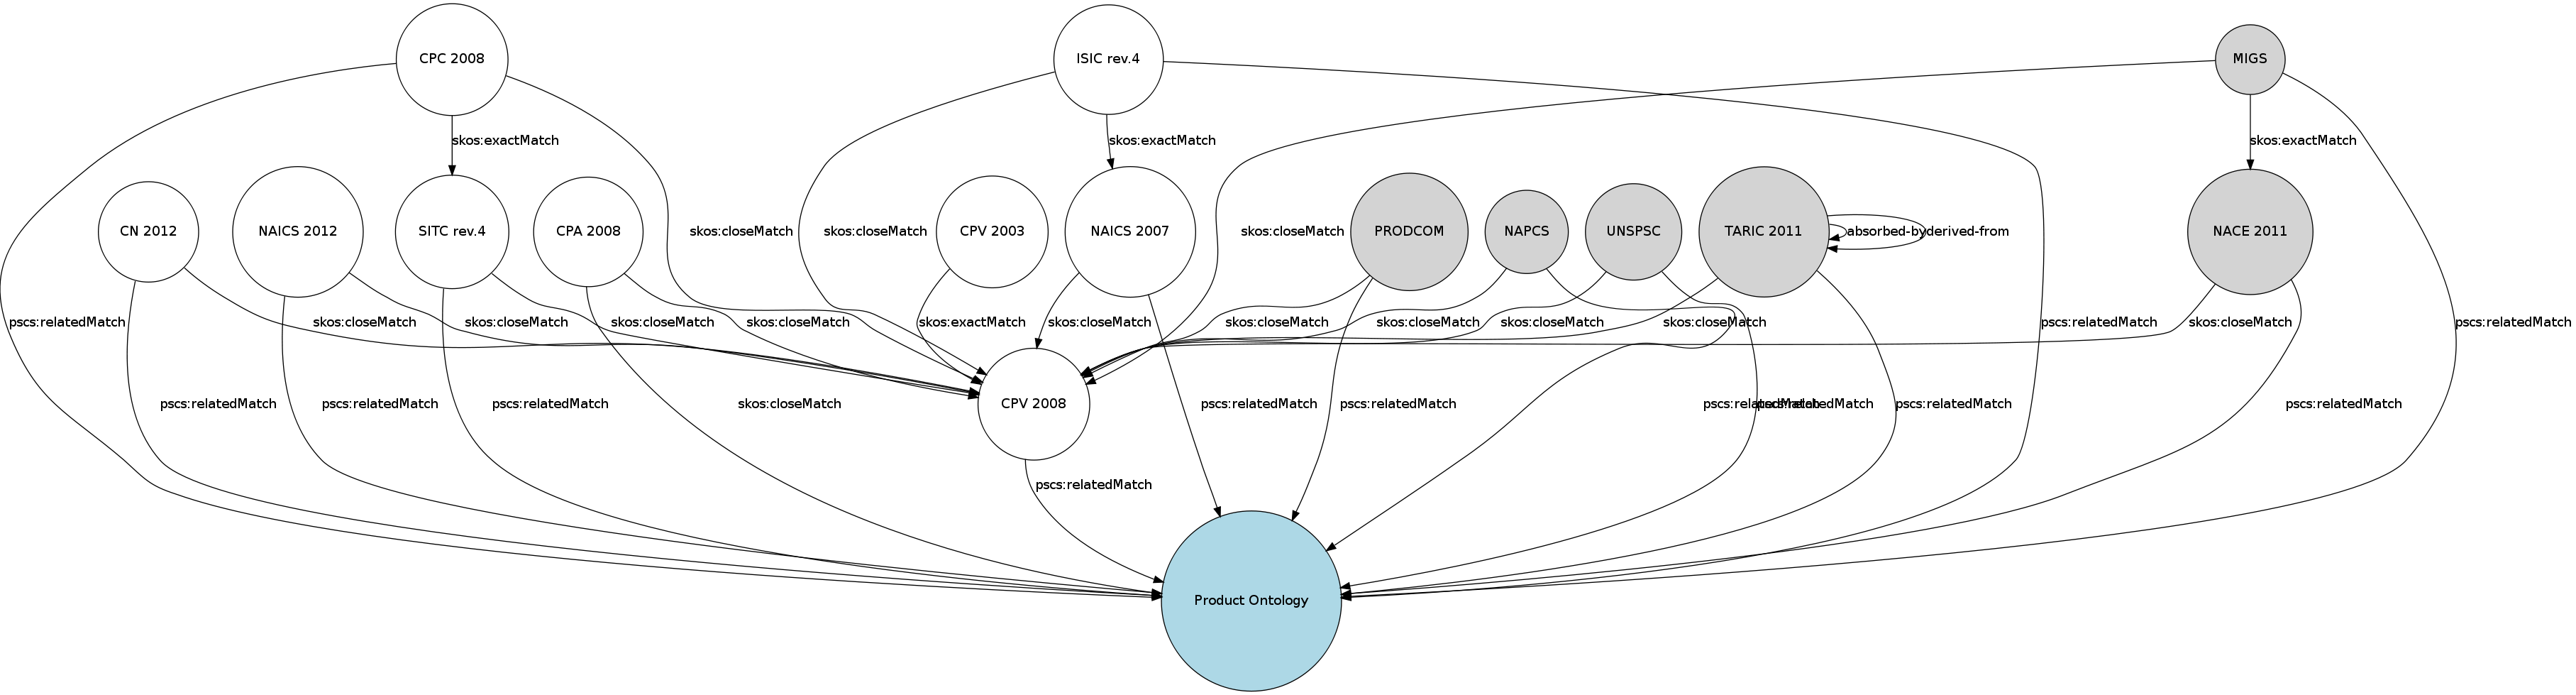
\includegraphics[width=18cm,angle=90]{./images/phd/pscs}
% \caption{Tarea $t_9$-Transformación de los Datos a RDF de las Organizaciones.}
% \label{fig:t9-orgs}
% \end{figure}

\subsubsection{Tarea $t_{10}$-Reconciliación de Entidades}
El diseño y ejecución de esta tarea ha sido descrito en la Sección~\ref{t8-orgs} ya que están 
estrechamente ligadas.

\subsubsection{Tarea $t_{16}$-Añadir metainformación a los recursos RDF}\label{t16-orgs}
Al igual que con las clasificaciones de productos, la metainformación cobra sentido a 
nivel de \dataset, ver Figuras~\ref{fig:orgs-ds},~\ref{fig:people-ds} y~\ref{fig:countries-ds}, ya que no se consideran cambios probables en un corto espacio de tiempo 
en cada una de las entidades gestionadas. En cualquier caso, tratándose de las organizaciones 
la ontología seleccionada para representar el modelo formal de los recursos ya recoge 
la posibilidad de añadir metainformación relativa a posibles eventos de cambios. Teniendo 
en cuenta que la información de las personas está asociada indisolublemente a las organizaciones, tampoco se considera necesario incluir un exceso de metainformación 
en cada uno de estos recursos. Finalmente y en el caso particular de los países, los cambios que se puedan 
producir constituirían una evolución real del \dataset para verificar que la información de todos los países 
sigue siendo congruente. Por ello, se ha seguido el modelo de incluir la metainformación a nivel de 
\dataset y no de recurso en particular. Continuando con los vocabularios seleccionados en los anteriores 
apartados, la especificación realizada por \gls{voID} cubre las necesidades de metainformación para representar 
datos de procedencia, licencia, etc.

\begin{figure}[!htp]
\begin{lstlisting} 
<http://purl.org/weso/eprocurement/organization/resource/ds>
      a       void:Dataset ;
      rdfs:label "Organizations dataset 2011"@en ;
      dcterms:author 
            <http://www.di.uniovi.es/~labra/labraFoaf.rdf#me> , 
	    <http://www.josemalvarez.es/foaf.rdf#me> ;
      dcterms:contributor
            <http://purl.org/weso/pscs/resource/10ders> ,
	    <http://rdfohloh.wikier.org/project/moldeas/rdf> ;
      dcterms:description "Dataset of organizations provided in 10ders project" ;
      dcterms:license <http://opendatacommons.org/licenses/by/1.0/> ;
      dcterms:modified "2011-12-10"^^xsd:date ;
      dcterms:publisher <http://www.josemalvarez.es/foaf.rdf#me> ;
      dcterms:source <http://purl.org/weso/pscs/resource/10ders> ;
      dcterms:title "Organizations dataset 2011" ;
      void:dataDump <http://purl.org/weso/eprocurement/organization/organization-10ders.ttl> ;
      void:exampleResource
        <http://purl.org/weso/eprocurement/organization/resource/org1> , 
	<http://purl.org/weso/eprocurement/organization/resource/org2> , 
	<http://purl.org/weso/eprocurement/organization/resource/org3> ;
      void:uriRegexPattern
        "http://purl.org/weso/eprocurement/organization/resource/.+" ;
      void:vocabulary org: , rdfs: , vcard: ;
      foaf:homepage <http://purl.org/weso> .
\end{lstlisting}
	\caption{Descripción del \dataset de Organizaciones.}
	\label{fig:orgs-ds}
\end{figure}
\cleardoublepage
\begin{figure}[!htp]
\begin{lstlisting} 
<http://purl.org/weso/eprocurement/organization/person/resource/ds>
      a       void:Dataset ;
      rdfs:label "People of the Organization"@en ;
      dcterms:author 
            <http://www.di.uniovi.es/~labra/labraFoaf.rdf#me> , 
	    <http://www.josemalvarez.es/foaf.rdf#me> ;
      dcterms:contributor
            <http://purl.org/weso/pscs/resource/10ders> ,
	    <http://rdfohloh.wikier.org/project/moldeas/rdf> ;
      dcterms:description "Dataset of people working on organizations provided in 10ders project" ;
      dcterms:license <http://opendatacommons.org/licenses/by/1.0/> ;
      dcterms:modified "2011-12-10"^^xsd:date ;
      dcterms:publisher <http://www.josemalvarez.es/foaf.rdf#me> ;
      dcterms:source <http://purl.org/weso/pscs/resource/10ders> ;
      dcterms:title "People of the Organization" ;
      void:dataDump <http://purl.org/weso/eprocurement/organization/person/person-organization-10ders.ttl> ;
      void:exampleResource
        <http://purl.org/weso/eprocurement/organization/person/resource/p1> , 
	<http://purl.org/weso/eprocurement/organization/person/resource/p2> , 
	<http://purl.org/weso/eprocurement/organization/person/resource/p3> ;
      void:uriRegexPattern
        "http://purl.org/weso/eprocurement/organization/person/resource/.+" ;
      void:vocabulary foaf: , org: , rdfs: , vcard: ;
      foaf:homepage <http://purl.org/weso> .
\end{lstlisting}
	\caption{Descripción del \dataset de Personas.}
	\label{fig:people-ds}
\end{figure}


\begin{figure}[!htp]
\begin{lstlisting} 
<http://purl.org/weso/eprocurement/country/resource/ds>
      a       void:Dataset ;
      rdfs:label "ISO 3166 Countries"@en ;
      dcterms:author 
            <http://www.di.uniovi.es/~labra/labraFoaf.rdf#me> , 
	    <http://www.josemalvarez.es/foaf.rdf#me> ;
      dcterms:contributor
            <http://purl.org/weso/pscs/resource/10ders> ,
	    <http://rdfohloh.wikier.org/project/moldeas/rdf> ;
      dcterms:description "Dataset of ISO 3166 Countries" ;
      dcterms:license <http://opendatacommons.org/licenses/by/1.0/> ;
      dcterms:modified "2011-12-12"^^xsd:date ;
      dcterms:publisher <http://www.josemalvarez.es/foaf.rdf#me> ;
      dcterms:source <http://purl.org/weso/pscs/resource/10ders> ;
      dcterms:title "ISO 3166 Countries1" ;
      void:dataDump <http://purl.org/weso/eprocurement/country/countries.ttl> ;
      void:exampleResource
        <http://purl.org/weso/eprocurement/country/resource/ES> , 
	<http://purl.org/weso/eprocurement/country/resource/BE> , 
	<http://purl.org/weso/eprocurement/country/resource/IT> ;
      void:uriRegexPattern
        "http://purl.org/weso/eprocurement/country/resource/.+" ;
      void:vocabulary geo: , rdfs: , dbpedia: ;
      foaf:homepage <http://purl.org/weso> .
\end{lstlisting}
	\caption{Descripción del \dataset de Países.}
	\label{fig:countries-ds}
\end{figure}



\subsubsection{Resultado Final y Ejemplos}
El resultado final del proceso de producción de \linkeddata, tras el análisis y ejecución 
de las tareas identificadas y del método de producción seleccionado, genera como resultado tres \datasets correspondientes 
a las entidades organización, persona y país mediante datos enlazados, en los cuales se pueden extraer las siguientes 
estadísticas de producción de datos, así como ejemplos de los recursos generados, ver Tabla~\ref{table:orgs-ejemplos}. Por otra parte, 
el aumento de la expresividad en el momento de realizar consultas se puede observar en la Figura~\ref{fig:orgs-sparql-query} en la 
cual se expresa la siguiente consulta:

\begin{Frame}
\textit{``Dame la forma de contacto de todas las organizaciones que han publicado anuncios de licitación en un determinado país.''}
\end{Frame}


\begin{longtable}[c]{|p{4cm}|p{3.5cm}|p{2cm}|p{2cm}|p{2.5cm}|} 
\hline
  \textbf{Conjunto de datos} & \textbf{Nº de Elementos}  &  \textbf{Ejemplo} &  \textbf{Tripletas} &  \textbf{Enlaces externos}  \\\hline
\endhead
Organizaciones & $50000$  & Figura~\ref{fig:orgs-example}   & $1150020$  & $50000$ (países)   \\ \hline
Personas & $50000$ &  Figura~\ref{fig:people-example}   & $900219$  & $50000$  (países)  \\ \hline
Países & $246$& Figura~\ref{fig:countries-example}      & $1756$  & $1779$ \\ \hline
\multicolumn{5}{|c|}{\textbf{Organizaciones Personas y Países} (total)} \\ \hline
Agregado & $100246$ &  N/A & $2051995$ & $101779$   \\ \hline
\hline
\caption{Estadísticas y Ejemplos de las Organizaciones.}\label{table:orgs-ejemplos}\\    
\end{longtable}

\begin{figure}[!htp]
\begin{lstlisting} 
SELECT DISTINCT * WHERE{
  ?org rdf:type org:FormalOrganization .
  ?org ref-country ?country.
  ?country rdfs:label ?labelCountry.
  FILTER (?country != <http://nuts.psi.enakting.org/id/ES>).  
  ?org org:hasSite ?site .
  ?org org:siteAddress ?vcard.
} LIMIT 100
\end{lstlisting}
	\caption{Ejemplo de consulta en SPARQL sobre los datos de Organizaciones.}
	\label{fig:orgs-sparql-query}
\end{figure}

\begin{figure}[!htp]
\lstinputlisting{examples/e-proc/country.ttl}
	\caption{Ejemplo final de un País.}
	\label{fig:countries-example}
\end{figure}


\begin{figure}[!htp]
\lstinputlisting{examples/e-proc/org.ttl}
	\caption{Ejemplo final de una Organización.}
	\label{fig:orgs-example}
\end{figure}

\begin{figure}[!htp]
	\lstinputlisting{examples/e-proc/person.ttl}
	\caption{Ejemplo final de una Persona.}
	\label{fig:people-example}
\end{figure}

\newpage

\subsubsection{Método de Producción de \linkeddata de Organizaciones}
Siguiendo las directrices señaladas en el análisis y diseño de entidades 
participantes en el modelado de organizaciones y la tabla de decisión~\ref{tabla:produccion}, el método semántico seleccionado 
para realizar la producción de datos enlazados es el $SPM_1$-``Transformación de datos a RDF'', ver Sección~\ref{spm-1}, en el que 
se transforman un conjunto de datos de entrada $\mathcal{G}$ a un \dataset RDF $\mathcal{D}$. Según la definición de método 
semántico de producción, realizada en la Sección~\ref{method-prod-def}, y el estudio de las organizaciones se pueden 
establecer los siguientes conjuntos:

\begin{itemize}
 \item $\mathcal{G}$ es el \dataset de entrada, conjunto de tuplas, conteniendo los datos de cada una de las organizaciones, las personas y los países. 
 \item $\mathcal{M}$ es el conjunto de \textit{mapeos}, ver Tabla~\ref{table:orgs-mappings}, extraídos según el análisis y diseño realizado en las secciones anteriores. Estos 
\textit{mapeos} son directamente expresables en la herramienta de transformación y toman como parámetros el valor de una de las tuplas de entrada (posición $X$) y la propiedad a generar.
 \item \textit{Dataset} \gls{RDF} $\mathcal{D}$ es el \dataset resultado, siguiendo el análisis y diseño realizado en las secciones anteriores y tras la ejecución 
de la tarea propia de transformación de datos.
\end{itemize}

\begin{longtable}[c]{|p{2cm}|p{8cm}|p{4cm}|} 
\hline
  \textbf{$\mathcal{M}$} &  \textbf{Propiedad} & \textbf{Valor} \\\hline
\endhead
 $m_1$ & \texttt{rdf:type} & \gls{URI} \\ \hline
 $m_2$ & \texttt{rdfs:label} & \texttt{xsd:string@lang}  \\ \hline
 $m_3$ & \texttt{org:purpose} & URI \\ \hline
 $m_4$ & \texttt{org:hasSite} & URI \\ \hline
 $m_4$ & \texttt{org:siteAddress} & URI  \\ \hline
 $m_5$ & \texttt{org:memberOf} & URI \\ \hline
 $m_6$ & \texttt{org:basedAt} & URI  \\ \hline
 $m_7$ & \texttt{ref-country} & URI \\ \hline  
 $m_8$ & \texttt{ref-dbpedia} & URI \\ \hline
 $m_9$ & \texttt{located-in}  & URI \\ \hline
 $m_{10}$ & \texttt{short-label}  & \texttt{xsd:string} \\ \hline   
 $m_{11}$ & \texttt{geo:lat}  & \texttt{xsd:double} \\ \hline
 $m_{12}$ & \texttt{geo:long}  & \texttt{xsd:double} \\ \hline   
 $m_{13}$ & \texttt{vcard:*}  & URI (incluyendo más \textit{mapeos} dependiendo de la información) \\ \hline         
\hline
\caption{Conjunto de \textit{mapeos} $\mathcal{M}$ para las Organizaciones.}\label{table:orgs-mappings}\\    
\end{longtable}

\subsection{Proceso de Publicación de \linkeddata de Organizaciones}
Evidentemente, la estrategia definida para todos los \datasets implicados en el proceso de contratación pública 
electrónica es común, por ello el proceso de publicación es homogéneo siguiendo la estructura definida 
en la Sección~\ref{sect:proceso-publicacion-ld}.

\subsubsection{Tarea $t_{14}$-Infraestructura para \linkeddata}
Nuevamente, la estrategia definida para todos los \datasets implicados en el proceso de contratación pública 
electrónica es común, por ello la infraestructura utilizada es la misma que la definida 
en la Sección~\ref{infraestructura-comun}.

\subsubsection{Tarea $t_{15}$-Acceso y formato en datos RDF}
De la misma forma que en el apartado anterior, el acceso y formato de datos \gls{RDF} para los datos contenidos y relativos 
a las organizaciones siguen el esquema proporcionado en la Sección~\ref{t15-comun}.

\subsection{Proceso de Consumo de Organizaciones}
El proceso de consumo de datos enlazados, según la definición realizada en la Sección~\ref{sect:proceso-consumo}, consiste en 
la reutilización de los datos enlazados para ser aplicados en la construcción de una nueva aplicación o servicio de valor 
añadido. En general, la reutilización más sencilla consiste en la representación gráfica de los recursos o la simple 
consulta con selección de formato de datos de acuerdo a las características de publicación utilizadas. En el caso 
que nos ocupa y teniendo en cuenta el objetivo de realización de un prototipo experimental de extracción de anuncios 
de licitación como demostrador del consumo de datos enlazados, se ha escogido el método semántico de consumo $SCM_2$-``\textit{Mapeo} a Lenguaje de Programación'', 
cuya descripción está disponible en la Sección~\ref{scm2-consumo}, orientado a obtener una representación de los recursos RDF en un 
lenguaje de programación (en este caso Java) como objetos de negocio. De acuerdo a este objetivo y a la definición del propio método 
es necesario definir:
\begin{itemize}
 \item El \dataset RDF $\mathcal{D}_{pub}$, es el conjunto de datos disponible tras aplicar el método de publicación.
 \item El conjunto $\mathcal{M}^1$, ver Tabla~\ref{table:orgs-consumo}, indica como transformar el \dataset anterior a la representación objetivo, objetos del lenguaje Java.
\end{itemize}

De esta manera, se obtienen una serie de objetos, $\mathcal{D}_{consum}$, con la información y datos necesarios, no se transforman necesariamente todos los datos disponibles en los recursos pertenecientes 
a  $\mathcal{D}_{pub}$, para ser reutilizados como objetos de negocio en un lenguaje de programación. Es conveniente señalar que el acceso a los datos se realiza a través 
de la consulta al \textit{endpoint} de \gls{SPARQL} ejecutando consultas \textit{SELECT} y \textit{DESCRIBE}.

\begin{longtable}[c]{|p{2cm}|p{4.5cm}|p{8cm}|} 
\hline
  \textbf{$\mathcal{M}^1$} &  \textbf{Propiedad} & \textbf{Tipo en Java} \\\hline
\endhead
 $m^1_1$ & URI recurso     		& \texttt{java.lang.String} \\ \hline
 $m^1_2$ & \texttt{rdf:type}      	& \texttt{org.weso.moldeas.to.{OrganizationTO, PersonTO, CountryTO}}\\ \hline
 $m^1_3$ & \texttt{rdfs:label} 		& \texttt{Map<String,String>} (lang, value) \\ \hline
 $m^1_4$ & \texttt{org:purpose} 	& \texttt{List<org.weso.moldeas.to.PurposeTO>} \\ \hline
 $m^1_5$ & \texttt{org:hasSite}    	& \texttt{org.weso.moldeas.to.SiteTO} \\ \hline
 $m^1_6$ & \texttt{org:siteAddres} 	& \texttt{org.weso.moldeas.to.SiteAddressTO}  \\ \hline
 $m^1_7$ & \texttt{org:memberOf} 	& \texttt{org.weso.moldeas.to.OrganizationTO}\\ \hline
 $m^1_8$ & \texttt{org:basedAt} 	& \texttt{org.weso.moldeas.to.SiteTO} \\ \hline
 $m^1_9$ & \texttt{ref-country} 	& \texttt{org.weso.moldeas.to.CountryTO} \\ \hline  
 $m^1_{10}$ & \texttt{ref-dbpedia} & \texttt{org.weso.moldeas.to.CountryTO}   \\ \hline
 $m^1_{11}$ & \texttt{located-in}    & \texttt{List<org.weso.moldeas.to.NUTSTO>} \\ \hline   
 $m^1_{12}$ & \texttt{short-label} & \texttt{java.lang.String}\\ \hline   
 $m^1_{13}$ & \texttt{geo:lat} and  \texttt{geo:long} & \texttt{com.javadocmd.simplelatlng.LatLng} \\ \hline   
 $m^1_{14}$ & \texttt{vcard:*} 		& \texttt{org.weso.moldeas.to.VcardTO} \\ \hline   
\hline
\caption{Conjunto de \textit{mapeos} $\mathcal{M}^1$ de consumo para las Organizaciones.}\label{table:orgs-consumo}\\    
\end{longtable}

\subsection{Proceso de Validación de Organizaciones}
La validación como proceso transversal en cualquier etapa dentro del ciclo de vida de datos 
enlazados debe realizarse con el objetivo de asegurar la calidad de los datos. De acuerdo a la 
definición realizada en la Sección~\ref{sect:validation}, este proceso consiste en la comprobación 
de que los recursos de un \dataset RDF cumplen ciertas características. Siguiendo con la estrategia marcada para 
todos los datos implicados en el proceso de contratación pública electrónica, la descripción completa de la validación de acuerdo 
a todas las características, se reseña en las Tablas de Validación disponibles en el Apéndice~\ref{tablas-validacion-apen}.

\subsubsection{Tarea $t_{12}$-Validación de Recursos RDF}
Al igual que en apartados anteriores, de acuerdo a la estrategia definida y con la definición realizada de esta tarea en la Sección~\ref{lod-t12}, 
se puede asegurar que la transformación de la información correspondiente de las organizaciones a la iniciativa \linkeddata cumple estrictamente los 
siguientes puntos:

\begin{itemize}
 \item Los datos \gls{RDF} son correctos ya que se han utilizado herramientas y \gls{API}s (Google \gls{Refine} y Jena) que aseguran 
la generación correcta de RDF.
 \item El dominio y rango en las propiedades es correcta, ya que se realiza la validación contra el modelo definido.
 \item Se ha establecido metainformación sobre la procedencia a nivel de \dataset.
 \item Todos los recursos transformados siguen la plantilla objetivo RDF.
\end{itemize}

\subsection{Proceso de Realimentación de Organizaciones}
Este proceso, según la definición realizada en la Sección~\ref{proceso-realimentacion}, busca la mejora 
y perfeccionamiento de los datos promocionados a RDF. Esta situación emerge en el momento en el cual 
los datos comienzan a ser reutilizados tanto por aplicaciones o servicios como por individuos. En el caso 
particular de las organizaciones y sus entidades relacionadas (personas y países) no se han llegado 
a reutilizar por terceras partes, por lo que la realimentación ha quedado restringida a la captura 
de fallos por la propia aplicación \gls{MOLDEAS}, tratándose en este caso de una forma de realimentación 
basada en \textit{Usuarios y Aplicaciones} y de carácter \textit{Actualización Ocasional}.

